\chapter{Implementation and Results}
The following sub chapters present the results of this master's thesis. First, requirements are summarized. Subsequently, the example computation of a Groth16 proof and verification is described in detail. The first artifact, the zero-knowledge decentralized application (zk-DApp) is demonstrated. The second artifact, an architecture proposal for zero-knowledge data structure of spare part certification and meta data information is introduced. Ultimately, artifacts are evaluated and a future outlook is provided.

\section{Summary of Requirements}
The requirements positioned in previous chapters (4 and 5) can be summarized as follows: 

\begin{enumerate}
    \item Zero-knowledge proof systems are identified to be a disruptive technology in the domain of blockchain-based research and development. One project requirement is to \textbf{accumulate knowledge and current research outcomes} in this field to extend expertise within RAPADO \citep{ZedelJ}. As an outcome to the extensive literature review, the Groth16 algorithm is introduced in detail by using an example calculation problem (6.2). In the step-wise computation, the problem is split and transformed to an arithmetic circuit, arriving at a R1CS. From this, the QAP is calculated. Additionally, tools, e.g, homomorphic hiding and elliptic curve pairing are introduced. Ultimately, following the Groth16 protocol, the key and proof generation, as well as verification mechanisms are illustrated.
    \item The requirement of \textbf{constructing a trade-off between privacy, confidentiality and transparency} arises from preliminary work in the project and at the department of information systems \citep{FornaconFrank, ZedelJ, semesterproject}. The use of blockchain-based solutions enables great transparency at the cost of confidentiality. With the constantly increasing awareness for data privacy, combined with trust issues and regulatory data confidentiality requirements in the industry, zero-knowledge proof systems have to be explored and utilized to secure adoption of project results and products in the future. The first minimal viable product (MVP) of the zk-DApp for MRO data attestations contributes to this goal and satisfies this requirement. The zk-DApp is organized as follows: the backend directory stores the json input schema, the solidity smart contracts, the circom circuit and corresponding generated files (6.2). The lib directory stores shared files between backend and frontend, as well as hashing functions used, e.g, in the circuit code. The UI directory finds the correct schema to be used and also stores a copy of the final protocol transcript key and the witness generating file. It also stores the frontend code for the landing page and all corresponding pages to submit, attest to, and verify MRO data.
    \item Current paper-based MRO documentation of aviation spare parts largely sets the requirement for \textbf{fraud-preventive verification mechanisms, enabled though effective data formats and digitization of spare part documents}. Fraud-preventive verification is covered via the zk-DApp. However, current data digitization efforts for spare part documentation need to be further addressed: the zero-knowledge data structure architecture enables consistent and temper-proof data storage via merkle trees, and proofs specific memberships, e.g., mechanics who worked at a specific part at a given time, in zero-knowledge.
\end{enumerate}

\begin{comment}
-research disruptive technologies and creating knowledge in the project: calculation example Groth16
-privacy/confidentiality vs transparency : zk-DApp
-need for fraud-preventive verification mechanism enabled through effective data formats digitization of aviation parts and document data: architecture



Notizen:

In den Ausblick der zk-dapp
-für einen part die schwellenwerte finden
-time since last service
-validation network as attester—>Übergang zum 2.artefakt 

-schwellenwerte ausgelesen werden
-aber auch die attester müssen ausgelesen werden

—>release certificate: Behörde
—> shop report: MRO Betrieb

-MRO KPIs: für den Handel, aus den MRO Daten ergeben, aus Privatsphäre/Transparenz requirement, ohne dass man Einsicht ins gesamte shop report geben will
\end{comment}

\section{Groth16 proof and verification}
Let us use an example to illustrate the underlying mathematical methods that are applied in zk-SNARK. The example calculation will use the knowledge of the coefficient assumption for simplification. In practice, the FFT is applied. First, the arithmetic circuit is transformed into a R1CS. The R1CS is used to obtain the QAP. Homomorphic hiding, elliptic curves and pairing-based cryptography are introduced in more detail and put in context for the next steps of the calculation. Finally, the Groth16 protocol is introduced: First, the key generation steps are explained. Second, the proof is generated. Lastly, the verification steps are illustrated. Formal definitions are found in 5.2.

Say we want to prove we know a secret x so that

\[x^3 + x + 5 = 35\]

In this case, our secret is x = 3.
In practice, we would use hiding and modular arithmetic instead of real numbers and calculations since these are easy to forge and find solutions to, which will make the proof useless. For R1CS and QAP we will proceed with real numbers to show the underlying mechanisms. The following will demonstrate how any computation that needs to be proven can be converted into polynomial format.

\subsubsection{Arriving at a R1CS}

A rank-1 constraint system is a mathematical format to help us reduce our problem into a less complex computational problem. First, we flatten the equation by writing a short program that would break down the different steps to solve the equation.

\begin{enumerate}
    \item \(sum1 = x * x\)
    \item \(y = sum1 * x\)
    \item \(sum2 = y + x\)
    \item \(out = sum2 + 5\)
\end{enumerate}

As shown above, we arrive at an arithmetic circuit with 4 gates and the solution variables
\[x = 3, y = 27, sum1 = 9, sum2 = 30, out = 35.\]

From this, we can construct the solution vector \(s\) , which has to start with a dummy variable of value 1, which we call \textit{one}.
Now, the solution vector \(s\) is
\begin{align}
    \Vec{s} &= \begin{pmatrix}
     one \\ x \\ out \\ sum1 \\ y \\ sum2
\end{pmatrix}
\end{align}
Each gate will be represented so that
\begin{align}
     \Vec{s}\cdot\Vec{a_i} * \Vec{s}\cdot\Vec{b_i} - \Vec{s}\cdot\Vec{c_i} = 0
\end{align}

Let us go through every gate and assign the values for a, b and c.
For the first gate \(sum1 = x*x\), the values of a, b and c are assigned as follows:
\begin{align*}
    a_1 &=\begin{bmatrix}
        0 & 1 & 0 & 0 & 0 & 0
    \end{bmatrix}
\end{align*}
\begin{align*}
    b_1&=\begin{bmatrix}
        0 & 1 & 0 & 0 & 0 & 0 
    \end{bmatrix}
\end{align*}
\begin{align*}
    c_1&=\begin{bmatrix}
        0 & 0 & 0 & 1 & 0 & 0
    \end{bmatrix}
\end{align*}

This is correct, because the dot product of s and a, multiplied by the dot product of a and b, subtracted by the dot product of s and c is 0 (6.2).

This procedure is applied to every gate. Let us show more complex gates to underline the calculation. For example, the third gate and the fourth gate. The third gate \(sum2=y+x\) could be approached as the first gate, by setting the variables in the equation to 1. However, this would not fulfill the equation shown in (6.2). Therefore, the correct values for \(a_3, b_3 \text{ and }c_3\) are
\begin{align*}
    a_3 &=\begin{bmatrix}
        0 & 1 & 0 & 0 & 0 & 0
    \end{bmatrix}
\end{align*}
\begin{align*}
    b_3&=\begin{bmatrix}
        1 & 0 & 0 & 0 & 0 & 0 
    \end{bmatrix}
\end{align*}
\begin{align*}
    c_3&=\begin{bmatrix}
        0 & 0 & 0 & 0 & 0 & 1
    \end{bmatrix}
\end{align*}

Here, we make use of the dummy vector \textit{one}, so that we can arrive at 
\[30 * 1 - 30 = 0.\]

The fourth gate \(out=sum2+5\) also has to be approached by holding true to the dot product equation in (6.2) as well. We have to make use of the dummy vector once again. Setting the values of \(one, sum2 \text{ and } out\)  to 1 will give us the following incorrect solution:
\begin{align*}
     \Vec{s}\cdot\Vec{a_4} * \Vec{s}\cdot\Vec{b_4} - \Vec{s}\cdot\Vec{c_4} \neq 0.
\end{align*}
The calculation shows \(30 * 1 - 35 \neq 0\), which means we need to add 5, so that the dot product of vector \(s \text{ and } a\) adds up to 35. Therefore, the values of \(a_4, b_4 \text{ and }c_4\) are as follows:
\begin{align*}
    a &=\begin{bmatrix}
        5 & 0 & 0 & 0 & 0 & 1
    \end{bmatrix}
\end{align*}
\begin{align*}
    b&=\begin{bmatrix}
        1 & 0 & 0 & 0 & 0 & 0 
    \end{bmatrix}
\end{align*}
\begin{align*}
    c&=\begin{bmatrix}
        0 & 0 & 1 & 0 & 0 & 0
    \end{bmatrix}
\end{align*}

By combining our results into matrices, we can set up the corresponding R1CS:

\begin{align}
A&=\begin{pmatrix}
    0 & 1 & 0 & 0 & 0 & 0 \\
    0 & 0 & 0 & 1 & 0 & 0 \\
    0 & 1 & 0 & 0 & 1 & 0 \\
    5 & 0 & 0 & 0 & 0 & 1
\end{pmatrix}
\end{align}
\begin{align*}
B&=\begin{pmatrix}
    0 & 1 & 0 & 0 & 0 & 0 \\
    0 & 1 & 0 & 0 & 0 & 0 \\
    1 & 1 & 0 & 0 & 0 & 0 \\
    1 & 0 & 0 & 0 & 0 & 0
\end{pmatrix}
\end{align*}
\begin{align*}
C&=\begin{pmatrix}
    0 & 0 & 0 & 1 & 0 & 0 \\
    0 & 0 & 0 & 0 & 1 & 0 \\
    0 & 0 & 0 & 0 & 0 & 0 \\
    0 & 0 & 1 & 0 & 0 & 0
\end{pmatrix}
\end{align*}

\subsubsection{From R1CS to QAP}

The R1CS shows three matrices \(A, B \text{ and }C\) representing the four gates each of length six. It is transformed into a QAP by expressing polynomials as sums of Lagrange Interpolation (chapter 5.2.2). This results in three sets of polynomials \(A_i(X), B_i(X) \text{ and }C_i(X)\) each consisting of six polynomials of degree three. In the following, we will summarize the reason of setting up a QAP instead of continuing with the R1CS. Lagrange Interpolation allows us to come up with polynomial coefficients, which represent each gate, when evaluated at an X in the range of number of constraints (gates). With X = 1, the Lagrange Interpolation can be explained quite well, because it means that we can just add up the coefficients of the polynomials in \(A_i(X), B_i(X) \text{ and }C_i(X)\). Each set of polynomial is built so that evaluated at a gate X, whereby X has to be in the range of the number of gates (constraints), will deliver the specific value of X and 0 for the other values in that specific range.\newline
The QAP for our example:
\begin{align*}
    A_i(X) \\
    \begin{bmatrix}
        -5.0 & 9.166 & -5.0 & 0.833 \\
        8.0 & -11.33 & 5.0 & -0.666 \\
        0.0 & 0.0 & 0.0 & 0.0 \\
        -6.0 & 0.5 & -4.0 & 0.5 \\
        4.0 & -7.0 & 3.5 & -0.5 \\
        -1.0 & 1.833 & -1.0 & 0.166
    \end{bmatrix} \\
\end{align*}
\begin{align*}
        B_i(X) \\
    \begin{bmatrix}
        3.0 & -5.166 & 2.5 & -0.333 \\
        -2.0 & 5.166 & -2.5 & 0.333 \\
        0.0 & 0.0 & 0.0 & 0.0 \\
        0.0 & 0.0 & 0.0 & 0.0 \\
        0.0 & 0.0 & 0.0 & 0.0 \\
        0.0 & 0.0 & 0.0 & 0.0
    \end{bmatrix}
\end{align*}
\begin{align*}
        C_i(X) \\
    \begin{bmatrix}
        0.0 & 0.0 & 0.0 & 0.0 \\
        0.0 & 0.0 & 0.0 & 0.0 \\
        -1.0 & 1.833 & -1.0 & 0.166 \\
        4.0 & -4.833 & 1.5 & -0.166 \\
        -6.0 & 9.5 & -4.0 & 0.5 \\
        4.0 & -7.0 & 3.5 & -0.5
    \end{bmatrix}
\end{align*}
The corresponding values in the matrices represent polynomial coefficients and shall be read from right to left, e.g. \(A1(X) = 0.833x^3 - 5x^2 + 9.166x -5\). For example:
\begin{align}
     X = 1 \\
    A1(1) = 0, A2(1) = 1, A3(1) = 0, A4(1) = 0, A5(1) = 0, A6(1) = 0
\end{align}
Comparing the results with the first vector a of the first gate, we see that the results represent the first gate.
For example, evaluating \(A, B \text{ and }C\) at X = 1 means to adding up the coefficients of the first polynomial of \(A\) , which will result in a value matching to the vector value in the first gate. Then, the next polynomial in A etc. It will result in a vector of length six and will be correct if the values match vector a from the first gate in our R1CS. The same is done by evaluating the polynomials with X, whereby X starts at 1 and ends at the number of gates, in our case \(X=\{1,2,3,4\}\).
However, it would be cumbersome to evaluate each constraint individually. This is why we can make use of the QAP to check whether the dot product equation of the polynomials will hold:
\begin{align}
    A_i(X)\cdot \Vec{s} * B_i(X)\cdot \Vec{s} - C_i(X)\cdot \Vec{s} = H(X) * Z(X)
\end{align}
Interestingly, the left side of the equation is our target polynomial \(T(X)\), which we want to proof.
Now, let's have a look at the right side of the equation in (6.6). \(Z(X)\) is known if we know the number of constraints. In Groth16, it is made available in the trusted setup. In this case, we have four gates, so we arrive at
\begin{align}
    Z(X) = (x-1)(x-2)(x-3)(x-4)
\end{align}
\(H(X)\) is the hiding of our initial minimal example, those input we don't want to share, but prove we know the solution to. What role hiding plays will be explained shortly. Now, we want to still finish looking at the equation in (6.6). In essence, we want to proof we know a polynomial and its solution, so that
\begin{align}
    T(X) / Z(X) = H(X)
\end{align}
Ultimately, in our example, \(H(X)\) is also a polynomial. We know the QAP is correct, if \(H(X)\) is a polynomial without remainder. In this example, the resulting
\[H(X) = -0.44x^3 + 17.055x^2 - 3.666x.\]

Practically, the coefficients of each polynomial in \(A_i(X), B_i(X) \text{ and }C_i(X)\) are publicly known. The same can be said for \(Z(X)\) through knowing the number of constraints (in this example we have four constraints). The prover can calculate the coefficients of \(H(X)\) by dividing T(X) / \(Z(X)\). However, there is no zero-knowledge yet, since the prover has to prove knowledge of vector \(s\) and \(H(X)\) without revealing it.
\newpage

\subsubsection{Hiding}
Zk-SNARKs are dependent on a trusted setup releasing these parameters. The goal is to prove knowledge of the polynomial \(H(X)\) with all its coefficients without disclosing any of this information. Therefore, the trusted setup also provides a random secret point \(P\). Note, that \(P\) is hashed, calculated once and deleted from memory. Depending on the number of constraints, a certain amount of \(P\) values are needed. In our example, we have four constraints, which need \(P = {1, P, P^2, P^3}\), whereby the value of \(P^3\) corresponds to the value of \(x^3\) when the polynomials are evaluated. The following values of \(P\) are provided

\begin{align}
    hh(1), hh(P), hh(P^2), ..., hh(P^\textsuperscript{(no. of constraints - 1)})
\end{align}

The trusted setup makes these values publicly available in the CRS.

With our previous knowledge, we know that the prove will consist of
\begin{align}
    \frac{hh[A(P)] * hh[B(P)] - hh[C(P)])}{hh[Z(P)]} = hh[H(P)]
\end{align}

The hidings of our polynomials are numbers, that currently can just be forged. The following will show how it can be proven that these numbers are hidings of the polynomials \(A(X)\), \(B(X)\) and \(C(X)\) in \(P\) which is not known to anybody. Furthermore, we need to prove that in order to arrive at \(A(X)\), \(B(X)\) and \(C(X)\), the same solution vector \(s\) was used (6.6). 

In order to approach the first problem, proving that the hidings of \(A(X)\),  \(B(X)\) and \(C(X)\) were actually calculated in \(P\), we need to "extend" \(P\) by the same number, namely \(u\). The CRS consists also of \(hh(u*P), hh(u*P^2), hh(u*P^3)\), etc., i.e., it consists of two sets of hidings. We know that \(A(X)\) is a linear combination of the values of vector s inserted into the polynomials A1, A2, A3, etc. of A. B calculating \(hh[A(P)]\) and \(hh[A(u*P)]\) and looking if \(hh[A(P)] = u * hh[A(u*P]\) holds true, shows that the hiding of \(A(X)\) calculated in \(P\)is indeed a result of linear combination of A1, A2, A3, etc. and the values of the vector s (6.6). All we did is to prove that the same sets of hidings of \(P\)were use to arrive at these numbers. The same is applied to the hidings of \(B(X)\), \(C(X)\) in P.

For the second problem, to prove the same values of vector s were used to arrive at the hidings of \(A(X)\), \(B(X)\) and C(X) in \(P\) a similar approach can be used. In our example, vector s has six solution variables. We use a new variable K as
\begin{align}
    K = K1 + K2 + K3 + K4 + K5 + K6
\end{align}
\begin{align*}
    K1 = A1(P) + B1(P) + C1(P)\\K2 = A2(P) + B2(P) + C2(P)
\end{align*}
\begin{center}
    ... \\
\end{center}
\begin{align*}
    K6 = A6(P) + B6(P) + C6(P)
\end{align*}
By checking that 
\begin{align}
    hh[K(P)] = one*hh[K1] + x * hh[K2] + out * hh[K3] + ... + sum2 * hh[K6],
\end{align}
we can prove that indeed the same coefficients of vector s were used. This way it is nearly impossible to come up with numbers that hold true for another \(P\)and to create proofs without the knowledge of the coefficients.

\subsubsection{Homomorphic Hiding}

\(y = hh(x)\) is a hashing function. It is collision resistant, i.e., one cannot guess anything of x from y. For zero-knowledge proofs, this property alone is not sufficient. The hashing function should also preserve algebraic structures, so the checks in , e.g., (6.10) can be performed. Let us divide the term \textit{Homomorphic Hiding} into two sections to explain in more detail.

A function \(y = hh(x) = e^x\) is homomorphic if
\begin{align}
    hh(a*x1 + b*x2) = e^\textsuperscript{a*x1+b*x2} = e^\textsuperscript{a*x1} * e^\textsuperscript{b*x2} = hh(x1)^a * hh(x2)^b
\end{align}
As seen in (6.13), the basic exponential laws hold. However, this function is not hiding, because one could calculate the logarithmic base e of x, because of working with only real numbers \begin{math}\mathbb{R}  
\end{math} so far.

We need to express variables in a finite field as of modulo p with p being a large prime. The finite field consists only of integer inputs in the range of 1 and some value p-2. This way, expressing values in modular arithmetic, nobody can guess or calculate our base e anymore. Now,
\begin{align}
    y = hh(x) = G^x,
\end{align}
where G is a value in the finite field \begin{math}\mathbb{F}_p\end{math} and y will always be expressed as modulo p.

With homomorphic hiding being introduced, we know all the tools being used to prove that we can calculate the equation in (6.8) with the polynomials from the QAP and the same values of vector s, without knowing any \(P\)and u * P. We know how the proof is calculated without revealing our solution vector s. The following deals with the verification if the above equations hold true, without revealing the solution vector s.

\subsubsection{Elliptic Curve Pairing}

The goal of PCP and pairing-based zero-knowledge algorithms is to create a succinct proof, that a defined computation with given inputs produces certain known outputs, without revealing any information about them and to show that the constraints of that computation hold. Eventually, we want to check if the following equality holds true, i.e., that after transforming our problem into polynomial structure, we know some polynomials so that

\begin{align}
    \frac{A(x) * B(x)}{Z(x)} = H(x) + C(x)
\end{align}

We have the polynomials \(A, B \text{ and }C\), not expressed in real numbers, but mapped to a finite field with a large prime number. We can calculate \(H(X)\) as in (6.8). Now, we are going to use generators for each of our polynomial to produce points on an elliptic curve. This is necessary to make use of pairing, which allows us to check if equations, e.g., (6.13), hold true without knowing the actual variable values in these equations. In the following, some preliminaries will be introduced to create a basis for the Groth16 CRS generation, and proofing and verification mechanism.

Elliptic curves are used to define collision resistant one-way functions, i.e., homomorphic hiding functions. An elliptic curve is a polynomial, e.g., the elliptic curve used in Bitcoin (Figure 1). 

\begin{figure}
\centering
\begin{minipage}{.5\textwidth}
  \centering
  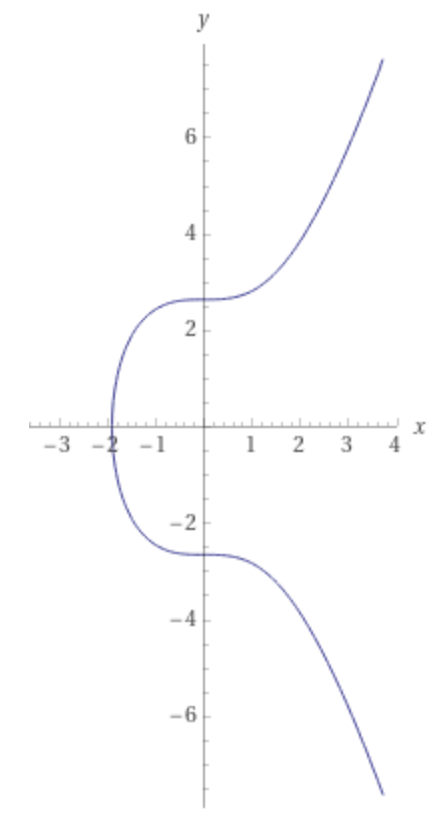
\includegraphics[width=.4\linewidth]{Pictures/bitcoinec.png}
  \caption{Figure 1:\ \(y^2 = x^3 +7\)}
  \label{fig:test1}
\end{minipage}%
\begin{minipage}{.5\textwidth}
  \centering
  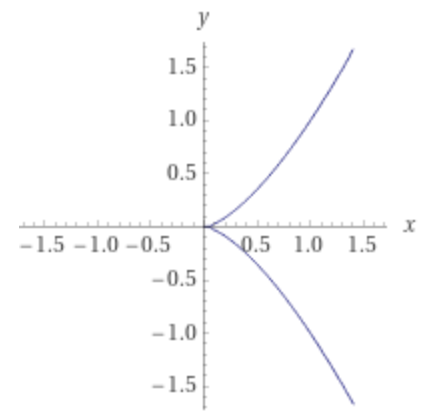
\includegraphics[width=.4\linewidth]{Pictures/y2x3.png}
  \caption{Figure 2:\ \(y^2 = x^3\)}
  \label{fig:test2}
\end{minipage}
\end{figure}

Elliptic curves are useful for zk-SNARKs because of the discrete logarithm problem, which is believed to be very hard to solve. Given a point \(g\) on the elliptic curve, and a multiple of that point, \(n*g\), it is impossible to solve n, even if \(g\) and \(n*g\) are given. In order to choose an elliptic curve that offers homomorphic hiding, we need to implement a mapping between our known numbers of the finite field \begin{math}\mathbb{F}_p\end{math} and a set of points on the elliptic curve (hidden space). Let \begin{math}\mathbb{F}_p\end{math} be a finite field of order p, whereby p is a large prime, e.g., if \(p=97\), then \begin{math}\mathbb{F}_p\end{math} \(=\{0, 1, 2, 3, ..., 96\}\) For this, we are going to take a generator point \(g = (x1,y1)\) that lies on the elliptic curve and multiply it with every element \({element}_i\) in \begin{math}\mathbb{F}_p\end{math}. For example, \(g + g = 2*g\) is calculated by putting a tangent line on \(g\), and wherever the line crosses the elliptic curve, we receive the result by using the opposite signs of that point. To arrive at \(2*g + g = 3*g\), the point \(2*g\) is used to draw a line to \(g\), see where the line further intersects with the elliptic curve, and use the opposite signs of that point to arrive at \(3*g\). This is repeated for every \(element\) in \begin{math}\mathbb{F}_p\end{math}. As a result, we have our finite field mapped to a hidden space on the elliptic curve. In summary, every \(element\) is hidden by
\begin{align}
    hh(element) = element * g
\end{align}
Additionally, we have to define what 0 and 1 are. The element 0 is the subtraction of a point on the elliptic curve, i.e., when point g goes to infinite. 1 is the point g itself.
Now, we have achieved homomorphic addition:
\begin{align}
    (A + B) \longrightarrow (A + B) * g = A*g + B*g
\end{align}

In order to use elliptic curve pairing to verify zk-SNARKs proofs, e.g., Groth16, we need to achieve a limited homomorphic multiplication operator. The hidden space is a group of points generated by the finite field elements and the generation point, \(g1\) on the elliptic curve. Now, we want to choose a subgroup \begin{math} \mathbb{G}_1\end{math} from that group. We choose that subgroup in a away that the number of elements we chose, \(r\), is a prime number too. Having found r, we can continue to choose the embedding degree of the elliptic curve. In Groth16, the proving key and verification key consist of \begin{math} \mathbb{G}_1\end{math} and \begin{math} \mathbb{G}_2\end{math} element. The embedding degree \(k\) has to be found in a way that \(p^k-1\ |\ r\), i.e., is a multiple of. Let us use a minimal example to show how to arrive at \begin{math} \mathbb{G}_1\end{math} and \begin{math} \mathbb{G}_2\end{math}.
Let us define an example base field \begin{math}\mathbb{F}_p\end{math} \(= \{0,1,2\}\) with \(p = 3\). We have found an embedding degree \(k=2\). In order to achieve our goal of creating a subgroup \begin{math} \mathbb{G}_2\end{math}, we need to extend our base field by a defining polynomial. This polynomial is of degree \(k\), and no element of our base field evaluates it to 0. In summary, we have:

\begin{align}
    \mathbb{F}_p = \{0,1,2\}, p = 3, k = 2
\end{align}

Defining polynomial for field extension \begin{math}\mathbb{F}_p^k\end{math}: 
\begin{align*}
    f(x) = z^2 +1 \\
    f(0) = 1\\
    f(1) = 2\\
    f(2) = 5 mod 3 = 2
\end{align*}

As shown in (6.18), none of the base field elements make f(x) evaluate to 0. In order to create the elements of the field extension \begin{math}\mathbb{F}_p^k\end{math}, we have to create all possible degree 2 polynomials out of the combinations of our base field \begin{math}\mathbb{F}_p\end{math}. For example, one possible polynomial with the coefficients from our base field is:

\begin{align}
    1*z^2+2*z+0 
\end{align}   
\begin{align*}
    (z^2+2*z)\mod (z^2+1) = 2*z-1\mod 3 = 2*z+2
\end{align*}
\(2*z+2\) is one element of the extension field \begin{math}\mathbb{F}_p^k\end{math}. In total, \begin{math}\mathbb{F}_p^k\end{math} has 9 elements, all calculated as in (6.18). In Summary, the elements of our extension field \begin{math}\mathbb{F}_p^k\end{math} are
\begin{align}
\{0, 1, 2, z, z+1, z+2, 2z, 2z+1, 2z+2\}
\end{align}

As shown in (6.20), the elements of the extension field are polynomials of degree up to \(k-1\). Addition and multiplication are defined in the way that coefficients are calculated \(\mod 3\) and polynomials \(\mod z^2+1\), the defining polynomial  
\(f(x)\) from (6.18).

Now, having our extension field, we can use it to create \begin{math}\mathbb{G}_2\end{math}, a subgroup of points of the same elliptic curve used for \begin{math}\mathbb{G}_1\end{math}, but with elements of \begin{math}\mathbb{F}_p^k\end{math}, instead of base field \begin{math}\mathbb{F}_p\end{math}. For this, we have to define points, whereby x and y coordinates are polynomials from \begin{math}\mathbb{F}_p^k\end{math}. \begin{math}\mathbb{G}_2\end{math} will consist of combinations from \begin{math}\mathbb{F}_p^k\end{math} in the form of \((x,y)\), which satisfy the elliptic curve. 

Pairings are bilinear maps that combine elements of two spaces to receive an element of a third space, e.g., matrix multiplication. In Groth16, the following pairing notation is used:

\begin{align}
    e: \mathbb{G}_1 \times \mathbb{G}_2 \to \mathbb{G}_T
\end{align}

The result of all steps performed previously is an incomplete homomorphic multiplication that enables us to check that the correct polynomial coefficients were used for \(A(x), B(X), \text{ and }C(x)\), as well as the same solution vector \(s\). It is incomplete, because not more than two elements can be multiplied. However, this just satisfies the use case for zk-SNARKs. 

\subsubsection{Groth16}

Preliminaries to understand the Groth16 protocol have been covered. In the following, we will describe the setup, proof, and verification steps in Groth16. The parameters are summarized in Table \ref{tab:Groth16Params}.

\setlength{\tabcolsep}{2ex}
\renewcommand{\arraystretch}{1.5}%
\begin{table}[hbt]
	\centering
	    \caption{Groth16 given parameters}
		\begin{tabular}{| m{0.35\linewidth} | m{0.6\linewidth} |}
		\hline
		\textbf{Parameter} & \textbf{Definition}\\ \hline
            \(n,m\) & number of constraints, number of variables\\ \hline
            \begin{math}\mathbb{F}_p\end{math} & finite field of prime order p\\ \hline 
            \begin{math}\mathbb{G}_1, \mathbb{G}_2, \mathbb{G}_T\end{math} & groups of points of prime order p satisfying an elliptic curve\\ \hline
            \begin{math}\mathbb{G}_1 \times \mathbb{G}_2 \to \mathbb{G}_T\end{math}& bilinear pairing \\ \hline
            \begin{math}g_T = e(g_1, g_2)\end{math}& generators with mapping \\\hline
            \begin{math}\bigl\{A_i(X), B_i(X), C_i(X)\bigl\}_{i=0}^m\end{math} & encoded computation as result of R1CS and QAP three sets of polynomials of degree \(n-1\)\\ \hline
            \(Z(x) = (x-1)*(x-2) * \newline (x-3)...(x-(n-1))\) &  minimal polynomial, known because n is known \\ \hline
            \(l\) & number of public inputs \\ \hline
            \((s_1,...,s_l)\) & elements of witness whose inputs are public \newline (e.g., out = 35 in our example) \\ \hline
            \((s_{l+1},s_{l+2},...s_m)\) & elements of witness for secret input x, with \(s_0 = 1\) \\ \hline
	\end{tabular}
\label{tab:Groth16Params}
\end{table}

\subsubsection{Key generation}

The proving and verification key are obtained from the Common Reference String (CRS) via multi-party computation. From \begin{math}\mathbb{F}_p\end{math}, a set of random values is generated. This toxic waste (tw), or trapdoor, must be secret and forgotten from memory, because knowledge of it enables forged proofs. Note, that \begin{math}\tau\end{math} is the random point \(P\) from our examples. From the toxic waste, polynomial \(L_i(x)\) is defined:
\begin{align}
    tw = (\alpha, \beta, \gamma, \delta, \tau) 
\end{align}
\begin{align*}
    L_i(x) = \beta * A_i(X) + \alpha * B_i(X) + C_i(X)
\end{align*}
The CRS consist of \begin{math} \sigma = ([\sigma_1]_1,[\sigma_2]_2)\end{math}, which are elements of \begin{math} \mathbb{G}_1, \mathbb{G}_2\end{math}.

\begin{align}
    [\sigma_1]_1 = 
    &\ [(\alpha, \beta, \gamma, \delta, \\
    &\ 1, \tau, \tau^2, \tau^3, ..., \tau^{n-1}, \\
    &\ \frac{L_0(\tau)}{\gamma}, ..., \frac{L_l(\tau)}{\gamma}, \\
    &\ \frac{L_{l+1}(\tau)}{\delta}, ..., \frac{L_m(\tau)}{\delta})]_1 
\end{align}
\begin{align*}
    [\sigma_2]_2 = [(\beta, \gamma, \delta, \ 1, \tau, \tau^2, \tau^3, ..., \tau^{n-1})]_2
\end{align*}

\begin{itemize}
    \item (6.23): elements of the toxic waste
    \item (6.24): powers of \begin{math}\tau\end{math} of degree up to \(n-1\)
    \item (6.25): the polynomial is chosen from the set of polynomials of \(A(X), B(X), C(X)\), which corresponds to the place of the public input of the solution vector. In our starting example, \(out = 35\) is the public input (since this is our only public input, \(l=1\)). The public input is at third place in s. Hence, \(A_3(X), B_3(X), C_3(X)\) are chosen, evaluated at \begin{math}\tau\end{math} and multiplied by \begin{math} \alpha, \beta\end{math} according to (24).
    \item (6.26): Same as (6.25), but for the non-public inputs of s. All elements of \begin{math} [\sigma_1]_1 \end{math} are \begin{math}\mathbb{G}_1\end{math} elements, e.g., \begin{math}\alpha_1 = g_1 * \alpha\end{math}.
\end{itemize}

The proving key consists of the following elements:
\begin{itemize}
    \item \([(\alpha, \beta, 1, \tau, \tau^2, \tau^3, ..., \tau^{n-1}, \frac{L_{l+1}(\tau)}{\delta}, ..., \frac{L_m(\tau)}{\delta})]_1\)
    \item \([(1, \gamma, \delta)]_2\)
    \item circuit information about the polynomials: \\
    \(A_0(X), A_1(X), ..., A_m(X)\),\\
    \(B_0(X), B_1(X), ..., B_m(X)\),\\
    \(C_0(X), C_1(X), ..., C_m(X)\),\\
    \(Z(x) = (x-1)(x-2)(x-3)...(x-(n-1))\)\\
\end{itemize}

The verification key consists of the following elements:
\begin{itemize}
    \item \([(1, \frac{L_0(\tau)}{\gamma}, ..., \frac{L_l(\tau)}{\gamma})]_1\)
    \item \([(1, \gamma, \delta)]_2\)
    \item precomputed pairing \([\alpha * \beta]_T\), which is a \begin{math}\mathbb{G}_T\end{math} element
\end{itemize}

\subsubsection{Generating the proof}

Two random numbers \(r, t\) are generated from \begin{math}\mathbb{F}_p\end{math}, that are used to compute

\begin{enumerate}
    \item \begin{math} A= \alpha + s_0*A_0(\tau) + s_1*A_1(\tau) + ... + s_m*A_m(\tau) + r\delta\end{math}
    \item \begin{math} B= \beta + s_0*B_0(\tau) + s_1*B_1(\tau) + ... + s_m*B_m(\tau) + t\delta\end{math}
    \item \begin{math} C= \frac{s_{l+1}L_{l+1}(\tau)}{\delta} + \frac{s_{l+2}L_{l+2}(\tau)} + ... +\frac{s_{lm}L_{lm}(\tau)}{\delta} + \frac{H(\tau)Z(\tau)}{\delta} + At + Br - rt\delta\end{math}
\end{enumerate}

The proof \begin{math}\pi\end{math} consists of two elements from \begin{math}\mathbb{G}_1\end{math} and one element from \begin{math}\mathbb{G}_2\end{math}:
\begin{align}
    \pi = ([A]_1, [B]_2, [C]_1)
\end{align}

\subsubsection{Verification}

In Groth16, three pairings are checked during verification. \begin{math}[\alpha * \beta]_T\end{math} is a precomputed pairing and is made available in the setup phase. The verification computation receives proof \begin{math} \pi\end{math} and accepts it only if the following equation holds:
\begin{align}
    [A]_1 * [B]_2 = [\alpha]_1[\beta]_2 + \bigl[\frac{s_0L_0(\tau)}{\gamma}+ \frac{s_1L_1(\tau)}{\gamma} + ... + \frac{s_lL_l(\tau)}{\gamma}\bigr]_1 * [\gamma]_2 + [C]_1 * [\delta]_2
\end{align}

As shown in (6.27), the following three pairings are needed to be checked:

\begin{itemize}
    \item \(e([A]_1, [B]_2)\)
    \item \begin{math}
        e(\bigl[\frac{s_0L_0(\tau)}{\gamma}+ \frac{s_1L_1(\tau)}{\gamma} + ... + \frac{s_lL_l(\tau)}{\gamma}\bigr]_1 , [\gamma]_2)
    \end{math}
    \item \begin{math}
        e([C]_1, [\delta]_2)
    \end{math}
\end{itemize}

Let us evaluate the verification equation in (6.27). The left hand side evaluates as follows:

\begin{equation*}
\begin{split}
    [A]_1 * [B]_2 = [A*B]_T &= [\alpha + s_0*A_0(\tau) + s_1*A_1(\tau) + ... + s_m*A_m(\tau) + r\delta]_1 \ *\\
    &\ \ \ \ [\beta + s_0*B_0(\tau) + s_1*B_1(\tau) + ... + s_m*B_m(\tau) + t\delta]_2 \\
    &= [(\alpha + A(\tau) + r\delta) * (\beta + B(\tau) + t\delta)]_T\\
    &= [\alpha * \beta]_T + [\alpha * B(\tau)]_T + [\alpha * t\delta]_T \ + [A(\tau) * \beta]_T \ + \\
    &\ \ \ \ [A(\tau) * B(\tau)]_T + [A(\tau) * t\delta]_T + [r\delta * \beta]_T + [r\delta * B(\tau)]_T +\\
    &\ \ \ \ [r\delta * t\delta]_T \\
    \\
    &= [A(\tau) * B(\tau)]_T \textcolor{blue}{\ +\ [\alpha * \beta]_T + [\alpha * B(\tau)]_T + [\alpha * t\delta]_T} \\
    &\ \ \textcolor{blue}{+ [A(\tau) * \beta]_T \ + [A(\tau) * t\delta]_T + [r\delta * \beta]_T + [r\delta * B(\tau)]_T} \\
    &\ \ \textcolor{blue}{+ [r\delta * t\delta]_T}
\end{split}
\end{equation*}

The right hand side evaluates to:
 \begin{equation*}
     \begin{split}
    &=[\alpha]_1[\beta]_2 + \bigl[\frac{s_0L_0(\tau)}{\gamma}+ \frac{s_1L_1(\tau)}{\gamma} + ... + \frac{s_lL_l(\tau)}{\gamma}\bigr]_1 * [\gamma]_2 + [C]_1 * [\delta]_2 \\
    &=[\alpha * \beta]_T + [(s_0L_0(\tau) + s_1L_1(\tau) + ... + s_lL_l(\tau))]_T + [(s_{l+1}L_{l+1}(\tau) + s_{l+2}L_{l+2}(\tau) + ... \\
    &\ \ \ + s_{lm}L_{lm}(\tau)) + H(\tau)Z(\tau) + At\delta + Br\delta - rt\delta\delta]_T
     \end{split}
 \end{equation*}

Now, we can replace A and B. We also see that the middle of the equation is \(L_i(\tau)\).
 \begin{equation*}
     \begin{split}
     &=[H(\tau) * Z(\tau) + C(\tau)]_T \textcolor{blue}{\ +\  [\alpha * \beta]_T + [\alpha * B(\tau)]_T + [\alpha * t\delta]_T + [A(\tau) * \beta]_T} \\
     &\ \ \ \textcolor{blue}{+ [A(\tau) * t\delta]_T + [r\delta * \beta]_T + [r\delta * B(\tau)]_T + [r\delta * t\delta]_T}
     \end{split}
 \end{equation*}

Eventually, we get the equality check we wanted to achieve (6.15). The use of the secret encoded values \(\alpha, \beta\) of the toxic waste (6.22) force the prover algorithm to use the same coefficients of the solution vector (witness) to compute \(A(X), B(X), C(X)\). \(\gamma, \delta\) ensure that the public inputs of order \(l\) are independent from the solution vector (witness). In order to achieve the zero-knowledge aspect, \(r, s\) are used to randomly shift the proof.

\section{Plonk-based zk-DApp}
The decentralized application for zero-knowledge MRO data attestation (zk-DApp) facilitates data entries and data sharing between MRO data owners (submitters) and aviation authorities (attesters) in zero-knowledge. This software artifact attempts to ensure compatibility between the lack of trust among industry participants and the need for data verification and transparency (trade-off between requirements within the project).
\subsubsection{Circom, snarkjs}
The zero-knowledge part of the zk-DApp is implemented via circom and snarkjs, which are developed by iden3. iden3 is an open-source project focused on scalable and distributed identity systems on zero-knowledge proofs, i.e., providing protocols, data structures, and modules. The current objectives include achieving self-sovereign identities free of charge, minimizing on-chain transactions, re-designing privacy with non-reusable proofs, creating complete products, e.g., user wallets, and focusing on community standardization \citep{iden3aboutus}. Circom is Rust-based and allows to write and compile arithmetic circuits. In circom, there is a data type called field elements, which are values modulo a large prime number and based on the BN128 elliptic curve by default \citep{circom} By compiling the circuit, R1CS files are generated: the constraint system in binary format, a symbols file for debugging, and files that are necessary to generate the witness. In order to compute the witness, an input file in json format needs to be specified, that contains the witness information. In the zk-DApp, the submitter enters the information to be verified, which is processed according to an input schema. The witness is computed and saved in a file format accepted by snarkjs. Snarkjs is a JavaScript library that continues with the outputs from circom and executes a specified zero-knowledge proof protocol, e.g., currently, Groth16, Plonk, and Fflonk are supported \citep{snarkjsdoc}. For this use case, snarkjs' plonk implementation is utilized. For the verification, as well as intermediate result hashes, a powers of tau file is utilized, so that the multi-party computation can be performed. In Groth16, it is utilized during the trusted setup (5.2.1). In plonk, this is the source of public randomness (5.2.2). Figure \ref{fig:zk-DAppgeneral} shows the main steps performed for a plonk-based zk-DApp. Plonk does not require a trusted ceremony for each circuit, i.e., the powers of tau ceremony is universal. After compiling the circuit and calculating the witness, the snarkjs plonk can be setup. A final protocol transcript key (zkey) is generated and verified. It is the zero-knowledge key that includes proving and verification key \citep{snarkjsdoc}. From the zkey, the verification key is exported in json format. With this verification key file, the final zkey file and the witness file, the proof file, and the file with the public inputs and outputs are generated. These two files and the verification key are used to verify the proof. The verifier is transformed into a smart contract (PlonkVerifier.sol), that is performing the verification. In order to utilize the PlonkVerifier smart contract that is exported in the previous step, an interface needs to be created (IPlonkVerifier.sol), which initiates verifyProof and outputs a true or false. The ZkDocument.sol smart contract, which stores user inputs, e.g., the commitments and trusted attesters, uses this interface to verify the proof and update the states of the smark contracts. With every user input, a witness and proof are calculated. The commitment is posted and the smart contracts updated. Once verified, the user interface (UI) shows an update, e.g., a green highlighting. 
\begin{figure}[hbt]
	\centering
		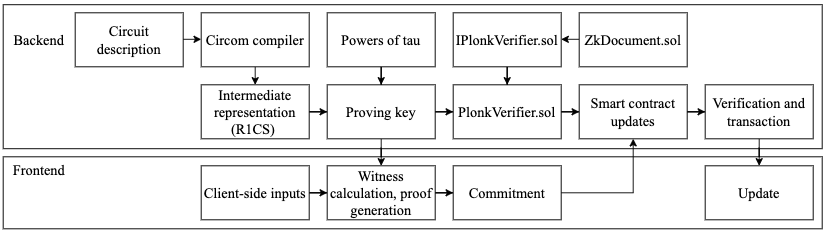
\includegraphics[width=1.0\textwidth]{Pictures/circom snarkjs process flow.png}
	\caption{plonk-based zk-DApp high-level process flow}
	\label{fig:zk-DAppgeneral}
\end{figure}
For deployment, broadcasting, and development, hardhat testnet is used. Metamask is used as crypto wallet browser plugin.

\subsection{Implementation and Results}
In the following, the different roles and the steps to be performed in the zk-DApp are described. First, the process flow and general functionalities are depicted. Second, important implementation logic and features are highlighted with references to the implementation code. Lastly, open items and limitations are discussed.

For the zk-DApp to start, the command \textit{yarn start} needs to be executed in the zkdocs-backend directory. It will start the hardhat test network and show a set of test accounts with private keys to use. These test accounts are also used for the accounts of the verifier, submitter and attesters. The next command in Figure \ref{fig:second-cmd} is also run in the same directory and deploys the schema for the MRO data entry. It triggers the circom and snarkjs ceremonies and shows the number of constraints, inputs, outputs, wires, and labels in the arithmetic circuit. Also, it shows that the corresponding R1CS, symbols and witness generating files are written successfully. Once, the setup is finished, the public keays of the deployer (submitter), plonk verifier (PlonkVerifier.sol smart contract address), and zkDoc (ZkDocument.sol smart contract address) are shown. The zkDoc public key needs to be parsed every time another set of inputs needs to be made, a verification needs to be performed, or to see the latest verification. In the end, the schema is created and the corresponding directories are listed. The UI can be started with the same command \textit{yarn start} in the zkdocs-ui directory.

\begin{figure}[hbt]
	\centering
		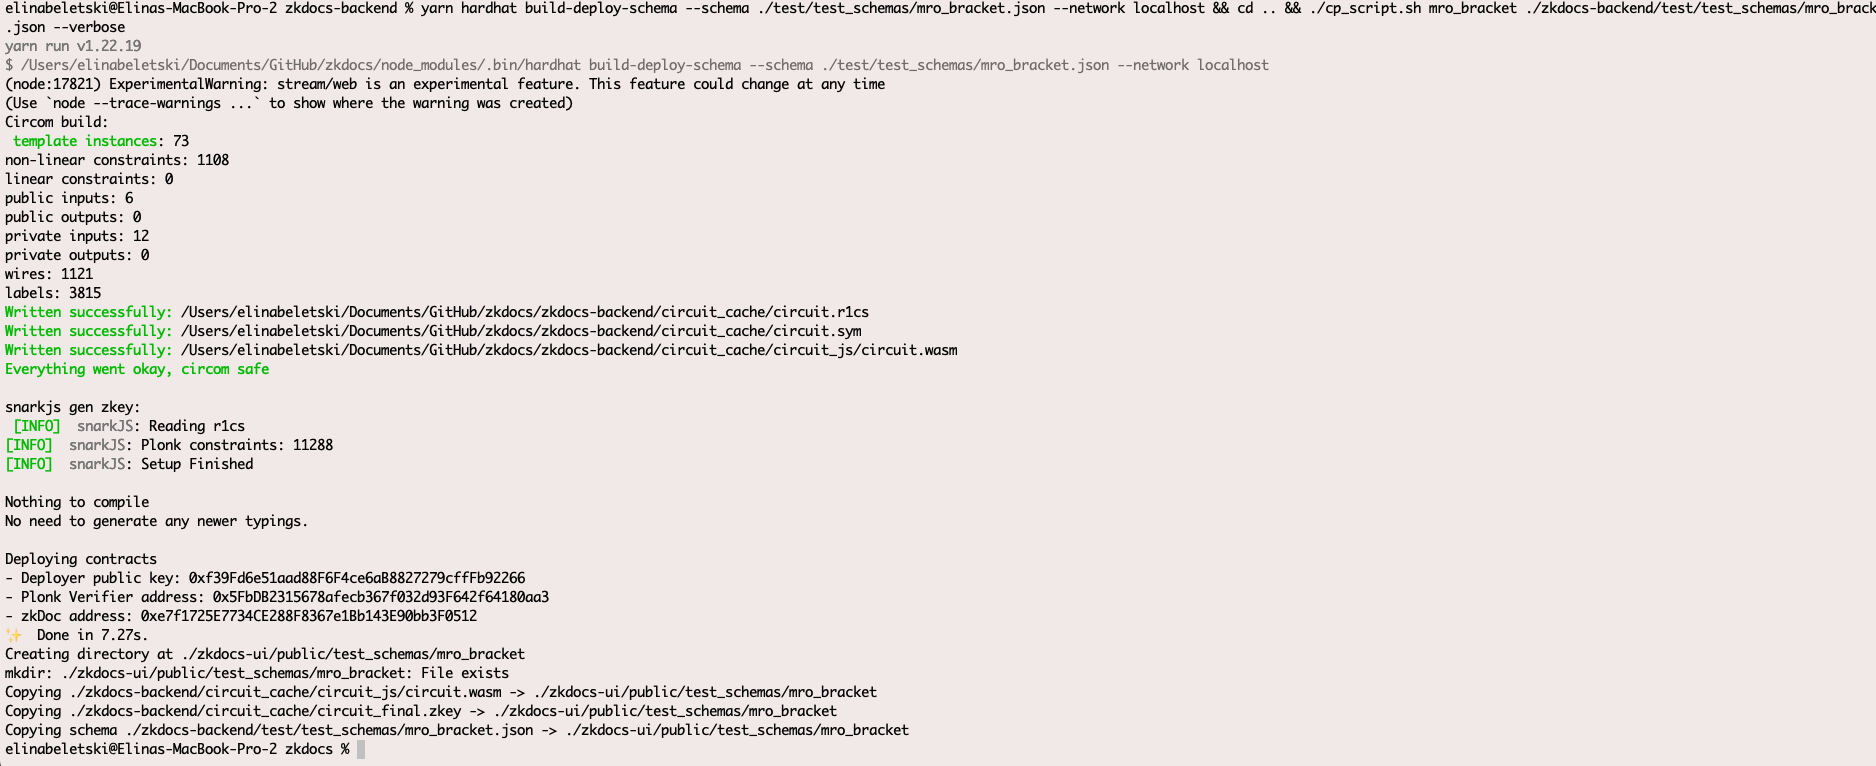
\includegraphics[width=1.0\textwidth]{Pictures/second-cmd.png}
	\caption{Initiating the deployment and plonk in circom, snarkjs in the zk-DApp backend}
	\label{fig:second-cmd}
\end{figure}

\subsubsection{Sequence of events}
In the zk-DApp, there are three roles: verifier, submitter, and attester. In this scenario, the verifier also acts as administrator, operating the zk-DApp. Hence, the administrator operates the schema with constraints, fields and the list of trusted institutions that are capable to attest in the zk-DApp. The submitter is in possession of MRO data, and seeks validation. The attester is assigned the task to view specific information shared with them and can validate it, i.e., attest to the data provided. The verifier can obtain the proof and verify it. Other stakeholders in the system can learn, that there is verified information, but do not learn anything besides its correctness. The following sequence of events refers to the landing page of the zk-DApp (Figure \ref{fig:landing-page}).
\begin{figure}[hbt]
	\centering
		
\includegraphics[width=1.0\textwidth]{Pictures/landingpage.png}
	\caption{zk-DApp landing page}
	\label{fig:landing-page}
\end{figure}
\begin{enumerate}
\item \textit{Fill Form}:
The submitter connects their wallet and can see an input mask for MRO data entries. In this first prototype, the submitter can enter the part identifier, flight hours, time since last service, and MRO cycles. Once the values are added, the submitter decides which authority needs to attest to the values, e.g., FAA/Unites States, EASA. If the constraints are met, the submitter generates the proof, which results in the following: first, the proof is generated and displayed. Second, there are communication links generated, that can be parsed in another browser tab. These links are specific to the respective attesters, so the data assigned to them can be viewed. In practice, this has to be realized via separate communication channels to alert attesters, once a new set of MRO data inputs was performed. The submitter commits to these entries and the proof on-chain. Now, the values can be viewed by the respective attester and validated.

\item \textit{Attest to MRO data}: The respective attester follows the attestation link, connects their wallet, and only sees the decrypted values of the data assigned to them for validation. The attester marks the data as true and commits the result. Once all attesters have successfully attested to the data, the verification can be initiated.

\item \textit{Verify Form}: Another user, e.g., the administrator, the submitter, or any dedicated user with the proof at hand, can perform the verification. The verifier connects their wallet and checks the attestations. The only information available is the green mark, that data has been successfully attested to, which fields have been attested to, and who attested to these fields and values. The values are shown in encrypted format. With the proof parsed, the verifier can verify and submit. If the attestations are correct, a bit will be flipped in the smart contract \citep{zkdocs}, and the verification is successfully performed.

\item \textit{View Verified}: Any participant can view the latest verified information. However, only the green mark is shown of whether the data is correct, the field names, and which trusted authority performed the attestation. The verifier and other participants do not learn anything besides that the information provided is correct and has been truthfully attested by a specific trusted institution.
\end{enumerate}
\subsubsection{Highlighted features}
The following features are described in more detail to illustrate the underlying functionality applied in the zk-DApp.

\begin{itemize}

\item The input for the circuit and witness calculation is processed through a schema. The json template can be seen as rule book for the input field and values, constraints, and trusted attesting addresses. \textit{ZkDocSchema.ts} uses the json template to define the schema. It sets valid operators, constraint types, and validates if the template matches to those. Some further value validations are build-in as well, e.g., checks for non-negative numbers. 

\item \textit{ZkDocGenerator.ts} acts as wrapper for circom and snarkjs. It contains all necessary commands to initiate the circuit, represent intermediate formats, e.g., R1CS, calculate the witness and the zero-knowledge key file, as well as exporting the verifier as smart contract. It generates the constraint string and looks up the field indices of the fields to attest in the schema. The circuit with its functionality is specified in \textit{circuit.circom}. It defines the constraints checks for each field, if the commitment matches the hashed commitment on-chain. During attestation, the assigned attester performs the decryption of the values locally.

\item The actual user input values are handled in the \textit{ZkDocument.sol} smart contract. It stores the selected attester addresses, the submitter's address, field commitments, and field indices to be attested to. For each field and value, a nonce is generated and the commitment scheme is initiated. The commitment scheme for each field is \textit{hash(value, nonce)}. The hashing algorithm used in the circuit is Poseidon. Due to its reduction of prover and verifier complexity, Poseidon is currently favored in research and development of zero-knowledge decentralized applications. Unlike other popular hashing functions, e.g., SHA-256, Poseidon is able to operate on smaller circuits and is adapted to finite fields \citep{poseidon}. It can add and remove trusted attesters from the list via \textit{(addValidInstitution, addValidInstitutions, removeValidInstitution)}. It makes sure, that only the attester specified by the submitter via mask entry is able to attest to the fields and values committed. During this check, it is also ensured that the field index of a attestation matches with the one specified during submission. Once the check is successfull, the bit is flipped to confirm correctness of the attestation. This procedure is applied to all field attestations at once via \textit{attestMultiple}. The function \textit{postFields} posts the commitments and checks that 1) the commitment length matches the number of fields, 2) that the correct number of institutions to perform attestations are in the commitment, and 3) that the commitment is unique and has not been posted previously. Through \textit{validateSubmitter} the public signal array for plonk verification is filled with the commitments. It checks that all fields have been attested to by the specified institutions. As described in the introduction of circom and snarkjs in 6.2, the verifier is transformed to a Solidity smart contract \textit{PlonkVerifier.sol}), containing the values and function logic needed for plonk verification. \textit{ZkDocument.sol} uses the interface to \textit{PlonkVerifier.sol}, the \textit{IPlonkVerifier.sol} to initiate the function \textit{verifyProof}, which verifies the proof. By using the interface, it is made sure that a specific standardized function from the generated \textit{PlonkVerifier.sol} is used (\textit{verifyProof}). This way of implementation makes sure, that the state of \textit{PlonkVerifier.sol} undergoes an actual change. In order to prevent client-side attacks, the schema hash, using the Keccak-256 hashing algorithm (part of SHA-3 Solidity family) is stored in \textit{ZkDocument.sol} as well. 

\item The UI finds the correct schema via the scheme hash stored, which is facilitated through \textit{SchemaUtils.ts}. From the schema hash, it obtains the corresponding schema and can utilize the files generated through the plonk procedure in circom and snarkjs (6.2).
\end{itemize}
\begin{comment}
ÜBERLEITUNG: 
- use case support system for predictive maintenance
- MRO KPIs are found in different documents, have to be attested by different institutions: e.g. shop report -->repair shop, release certificate-->aviation authority
- also for trading this is important information 
- this use case resulted from requirement privacy and transparency as well as trading of parts
- assumption: data is available
- überleitung zur daten architektur: automatic verification of part id and its true existence through merkle tree zk verification
\end{comment}

\section{Zero-Knowledge Data Structure}
-create a architecture for verification mechanisms in Rapado, based on Sedlmeier, Völter, Strüker (2021):
-->proof membership in a merkle tree? data structure of parts, certificates

- Campanelli et al 2022: improvement on zkSNARKS with Merkle Trees -->HARISA, could be used for the architecture

- build zk DAPP for document verification with circom snarkjs on hardhat test network
- maybe use snarkjs Groth16 first and then PLONK as future outlook, when TurboPLONK support will come in snarkjs

\section{Evaluation}
\begin{comment}
- how fast is the zk-DApp with plonk on my PC?
- why is the architecture good -->because it tackles the assumptions that are made for the zk-DApp and focuses on another big requirement in the project: the data digitization approach
- comparison of groth16 and plonk performance
- limitations of the implementation
- future outlook with turboplonk

content:
- data has to be made more available: automatic part id verification, automatic assignment of attesters according to fields (e.g. MRO cycles always done by repair shop)
- also automatic threshold identification according to part id and part description: e.g. a turbine needs another threshold than a wing
- data structure will dictate industry effectiveness of zero-knowledge proof implementations in the project as well as adoption
- zk-DApp flexible and easy to adapt to further business cases
- the data structure verification with zero-knowledge proposes another way of making use of ZKP for the requirement to create a industry standard for MRO data digitization and verification
\end{comment}


